\begin{figure*}[h]
    \centering
    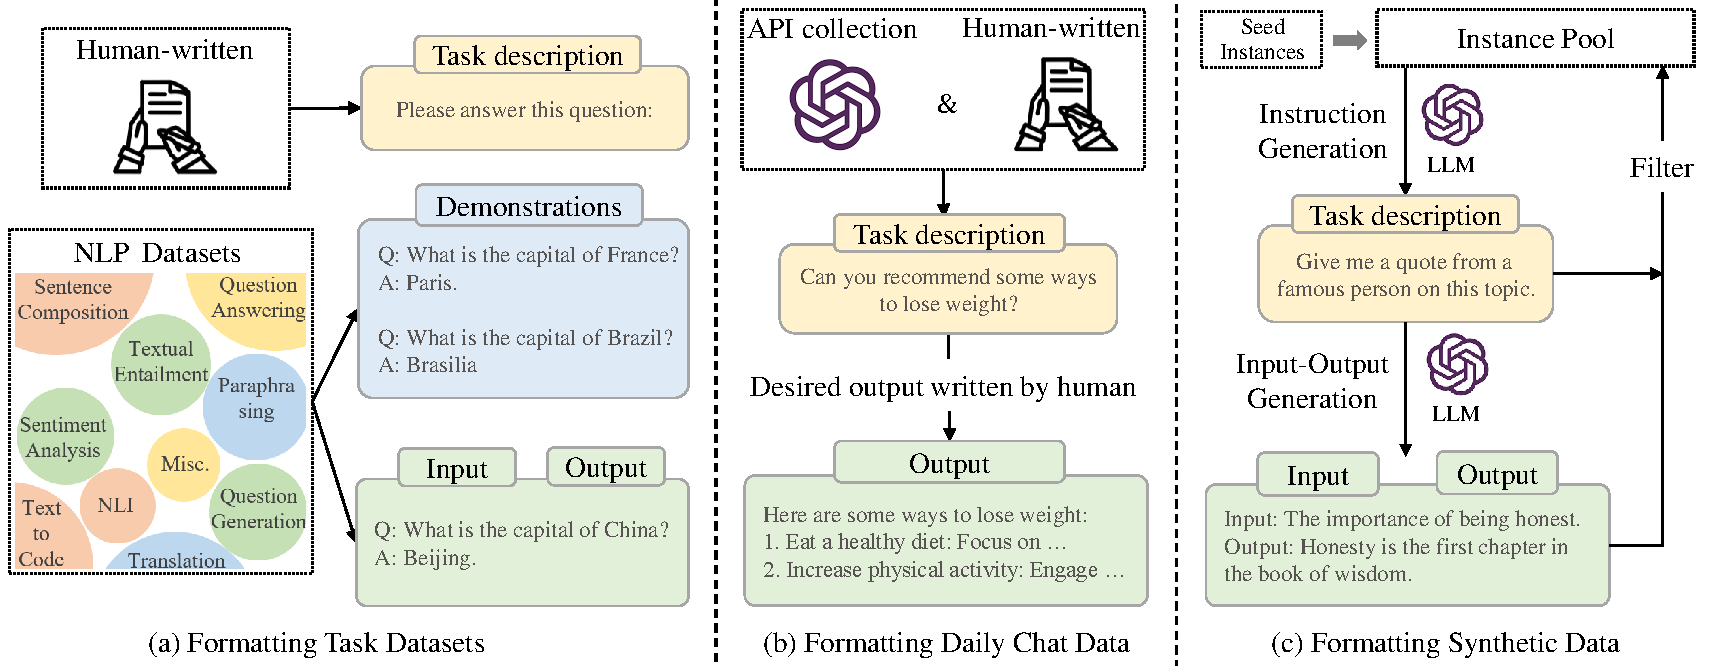
\includegraphics[width=1\textwidth]{images/Instruction-Tuning-new.pdf}
    \caption{An illustration of instance formatting and three different methods for constructing the instruction-formatted instances. }
    \label{fig:instruction-tuning}
\end{figure*}



\subsection{Instruction Tuning}
\label{sec-instruction}
In essence, instruction tuning is the approach to fine-tuning  pre-trained  LLMs on a collection of formatted instances in the form of natural language~\cite{Wei-ICLR-2022-Finetuned}, which is highly related to supervised fine-tuning~\cite{Ouyang-arxiv-2022-Training} and multi-task prompted training~\cite{Sanh-ICLR-2022-Multitask}. %
In order to perform instruction tuning, we first need to collect or construct instruction-formatted instances. 
Then, we employ these formatted instances to fine-tune LLMs in a supervised learning way (\eg training with the sequence-to-sequence loss). 
After instruction tuning, LLMs can demonstrate superior abilities to generalize to unseen tasks~\cite{Wei-ICLR-2022-Finetuned,Sanh-ICLR-2022-Multitask,Chung-arxiv-2022-Scaling}, even in a multilingual setting~\cite{Muennighoff-2022-arxiv-Crosslingual}. 


A recent survey~\cite{Lou-arXiv-2023-Is} presents a systematic overview of the research on instruction tuning. In comparison to that, we mainly focus on the effect of instruction tuning on LLMs and provide detailed guidelines or strategies for instance collection and tuning. In addition, we also discuss the use of instruction tuning for satisfying the real needs of users, which has been widely applied in existing LLMs, \eg InstructGPT~\cite{Ouyang-arxiv-2022-Training} and GPT-4~\cite{OpenAI-OpenAI-2023-GPT-4}.



\subsubsection{Formatted Instance Construction}\label{sec-instruction-formatted} 
Generally, an instruction-formatted instance consists of a task description (called an \emph{instruction}), an optional input, the corresponding output, and a small number of demonstrations (optional).
As important public resources, existing studies have released a large number of labeled data formatted in natural language (see the list of available resources in Table~\ref{tab:instruction-collection}) as introduced in Section~\ref{sec:it-dataset}. 
Next, we introduce three major methods for constructing formatted instances (see an illustration in Figure~\ref{fig:instruction-tuning}) and then discuss several key factors for instance construction.  



\paratitle{Formatting NLP Task Datasets.} 
Before instruction tuning was proposed, several early  studies~\cite{Liu-ACL-2019-Multi,Aghajanyan-EMNLP-2021-Muppet,Tang-arxiv-2022-MVP} collected the instances from a diverse range of traditional NLP tasks (\eg text summarization, text classification, and translation) to create supervised multi-task training datasets. 
As a major source of instruction tuning instances, it is convenient to format these multi-task training  datasets with natural language task descriptions. 
Specifically, recent work~\cite{Wei-ICLR-2022-Finetuned,Sanh-ICLR-2022-Multitask,Ouyang-arxiv-2022-Training,Wang-EMNLP-2022-Super}  augments the labeled datasets with human-written task descriptions, which instructs LLMs to understand the tasks by explaining the task goal.  %
For example, in Figure~\ref{fig:instruction-tuning}(a),  a task description ``\emph{Please answer this question}'' is added for each example in the question-answering task. 
After instruction tuning, LLMs can generalize well to other unseen tasks by following their task descriptions~\cite{Wei-ICLR-2022-Finetuned,Sanh-ICLR-2022-Multitask,Chung-arxiv-2022-Scaling}. 
In particular, it has been shown that instructions are the crucial factor in task generalization ability for LLMs~\cite{Wei-ICLR-2022-Finetuned}:  
by fine-tuning the model on labeled datasets with the task descriptions removed, it results in a dramatic drop in model performance.
To better generate labeled instances for instruction tuning, a crowd-sourcing platform, PromptSource~\cite{Bach-ACL-2022-PromptSource} has been proposed to effectively create, share, and verify the task descriptions for different datasets.  
To enrich the training instances, several studies~\cite{Sanh-ICLR-2022-Multitask,Tang-arxiv-2022-MVP,Longpre-arxiv-2023-The} also try to invert the input-output pairs of existing instances with specially designed task descriptions for instruction tuning. For instance, given a question-answer pair, we can create a new instance by predicting the answer-conditioned question (\eg \emph{``Please generate a question based on the answer:''}). %

\paratitle{Formatting Daily Chat Data.}
Despite that a large number of training instances have been formatted with instructions, they mainly come from public NLP datasets, either lacking instruction diversity or mismatching with real human needs~\cite{Ouyang-arxiv-2022-Training}.   
To overcome this issue, InstructGPT~\cite{Ouyang-arxiv-2022-Training} proposes to take the queries that real users have submitted to the OpenAI API as the task descriptions.  %
Additionally, to enrich the task diversity, human labelers are also asked to compose the instructions for real-life tasks, including open-ended generation, open question answering, brainstorming, and chatting. 
Then, they let another group of labelers directly answer these instructions as the output.
Finally, they pair one instruction (\ie the collected user query) and the expected output  (\ie the human-written answer) as a training instance.
Note that InstructGPT also employs these real-world tasks formatted in natural language for alignment tuning (discussed in Section~\ref{sec-alignment}). 
Further, GPT-4~\cite{OpenAI-OpenAI-2023-GPT-4} has designed potentially high-risk instructions and guided the model to reject these instructions through supervised fine-tuning for safety concerns. 
{Considering the absence of high-quality public chat data, several studies have also collected  users' chat requests as input data,  and then utilized ChatGPT or GPT-4 to generate responses as output data. A notable example of such a dataset is the conversational data from ShareGPT~\cite{ShareGPT}. Additionally, Dolly~\cite{Conover-2023-arxiv-Dolly} and OpenAssistant~\cite{kopf-arxiv-2023-openassistant} have further released their conversation data, which has been carefully labeled by human annotators to attain a high level of quality.}



\paratitle{Formatting Synthetic Data.}
To reduce the burden of human annotation or manual collection, several semi-automated approaches~\cite{Wang-arXiv-2022-Self} have been proposed for constructing instances by feeding existing instances into LLMs to synthesize diverse task descriptions and {instances}. As illustrated in Figure~\ref{fig:instruction-tuning}(c), the Self-Instruct method only needs 175 instances as the initial task pool. Then, they randomly select a few instances from the pool as demonstrations and prompt a LLM to generate new instructions and corresponding input-output pairs. After the quality and diversity filtering, newly generated instances would  be added into the task pool. Hence, the synthetic method is an effective and economical way to generate large-scale instruction data for LLMs. 
{However, the instances generated by the Self-Instruct method might be  simplistic or lack the diversity. To improve the quality of  synthetic int ructions,  WizardLM~\cite{Xu-arxiv-2023-WizardLM} introduces Evol-Instruct by proposing in-depth and in-breadth evolving to enrich the complexity and diversity of the instances. Furthermore, Self-Align~\cite{Sun-arxiv-2023-Principle} establishes multiple human-aligned principles to filter the synthesized instances. It then employs these instances to train a LLM in order to yield more aligned instances. To enhance the quality of the instance output, researchers directly adopt human-written texts as the output and synthesize corresponding instructions using ICL examples~\cite{Li-arxiv-2023-Self}.}





\paratitle{Key Factors for Instance Construction.}
The quality of instruction instances has an important impact on the performance of the model. 
Here, we discuss some essential factors for instance construction. 

$\bullet$ \emph{Scaling the instructions.} 
It has been widely shown that scaling the number of tasks can largely enhance the generalization ability of LLMs~\cite{Wei-ICLR-2022-Finetuned,Sanh-ICLR-2022-Multitask,Wang-EMNLP-2022-Super}. 
With the increasing of the task number, the model performance initially shows a continuous growth pattern, while the gain becomes negligible when it reaches a certain level~\cite{Wang-EMNLP-2022-Super,Chung-arxiv-2022-Scaling}. 
A plausible speculation is that a certain number of representative  tasks can provide relatively sufficient  knowledge and adding more tasks  may not bring additional gains~\cite{Chung-arxiv-2022-Scaling}.
Also,  it is  beneficial to enhance the diversity of the task descriptions in several aspects, such as length, structure, and creativity~\cite{Sanh-ICLR-2022-Multitask}.
As for the number of instances per task, it has been found that a small number of instances can usually saturate the generalization performance of the model to perform a specific task~\cite{Wei-ICLR-2022-Finetuned,Chung-arxiv-2022-Scaling}.
{Specially, several recent work~\cite{zhou-arxiv-2023-lima,Chen-arxiv-2023-AlpaGasus} has explored the effect of fine-tuning with a small amount of high-quality instruction data (\eg one or a few thousand instances),  showing very promising results on the evaluation tasks.  
In contrast, another line of studies continue to explore the scaling effect of instruction data~\cite{Mukherjee-arxiv-2023-Orca,YuLan-Chat}. For example, Orca~\cite{Mukherjee-arxiv-2023-Orca} scales up the synthesized instances to 5 million with step-by-step explanations, and it achieves superior performance across a wide range of tasks compared to the methods tuned with instruction  data.}





$\bullet$ \emph{Formatting design.}
As an important factor, the design of natural language format also highly impacts the generalization performance of LLMs~\cite{Wang-EMNLP-2022-Super}.
Typically, we can add task descriptions and optional demonstrations to the input-output pairs of existing datasets, where the task description is the most key part for LLMs to understand the task~\cite{Wang-EMNLP-2022-Super}. 
Further, it can lead to substantial improvements by using an appropriate number of exemplars as demonstrations~\cite{Chung-arxiv-2022-Scaling}, which also alleviates the model sensitivity to instruction engineering~\cite{Wei-ICLR-2022-Finetuned,Chung-arxiv-2022-Scaling}. 
However, incorporating other components (\eg things to avoid, reasons, and suggestions) into instructions may have a negligible or even adverse effect on the performance of LLMs~\cite{Mishra-ACL-2022-Cross, Wang-EMNLP-2022-Super}. 
Recently, to elicit the step-by-step reasoning ability of LLMs, some work~\cite{Chung-arxiv-2022-Scaling}  proposes to include chain-of-thought (CoT) examples for some reasoning datasets, such as arithmetic reasoning.
It has been shown that fine-tuning LLMs with both CoT and non-CoT examples can lead to a good performance across various reasoning tasks,  including those that require multi-hop reasoning ability (\eg commonsense question answering and arithmetic reasoning) as well as those without the need for such a reasoning  way (\eg sentiment analysis and  extractive question answering)~\cite{Chung-arxiv-2022-Scaling,Iyer-arxiv-2022-OPT}.


To summarize, diversity and quality of instructions seem to be more important than the number of instances~\cite{zhou-arxiv-2023-lima} since the well-performing  InstructGPT~\cite{Ouyang-arxiv-2022-Training} and LLaMA-2-Chat~\cite{Touvron-2023-llama2-arxiv} utilize fewer but more diverse instructions (or instances) than the Flan-series LLMs~\cite{Wei-ICLR-2022-Finetuned,Chung-arxiv-2022-Scaling}. However, a large amount of training data may compensate for the absence of high-quality data~\cite{Mukherjee-arxiv-2023-Orca}.
Further, it is more useful to invite labelers to compose human-need tasks than using  dataset-specific tasks. However, it still lacks general guidelines to  annotate human-need instances, making the task composition somehow heuristic. 
To reduce human efforts, we can either reuse existing formatted datasets (Table~\ref{tab:instruction-collection}) or automatically construct the instructions using existing LLMs~\cite{Wang-arXiv-2022-Self}. We conduct a preliminary experiment to show the effectiveness of different construction methods in Section~\ref{instruction-results}.


\begin{table*}[t]
    \centering
    \caption{Basic statistics of the required number of GPUs, tuning time, batch size (denoted as BS) per device (full tuning and LoRA tuning), and inference rate (the number of generated tokes per second). Our experiments are conducted based on two Linux servers having 8 A800-80G SXM4 GPUs with 6 NVSwitch and 8 3090-24G GPUs, respectively. {The major difference between A800 and A100 lies in the NVLink interconnect speed. Thus, our estimations about training and inference efficiency would be slightly improved for A100, while the rest memory consumption would remain the same.}  
    {
    For full tuning experiments, we use data parallel training, ZeRO Stage 3, BF16, and gradient checkpointing. Additionally, the LoRA tuning can be executed on one 80G GPU utilizing INT8 quantization with the rank setting set to 16. {All the experiments are conducted with Alpaca-52K dataset by  training LLaMA models three epochs.} The max sequence length for both training settings is set to 512. The inference experiments are performed with the batch size set to 1.}
    }
    \renewcommand\tabcolsep{2.5pt}
    \begin{tabular}{c|ccc|ccc|cc|cc|cc}
    \toprule
    \multirow{2}{*}{\textbf{Models}} & \multicolumn{3}{c|}{\textbf{A800 Full Training}} & \multicolumn{3}{c|}{\textbf{A800 LoRA Training}} & \multicolumn{2}{c|}{\textbf{A800 Inference (16-bit)}} & \multicolumn{2}{c|}{\textbf{3090 Inference (16-bit)}} & \multicolumn{2}{c}{\textbf{3090 Inference (8-bit)}} \\
    & \#GPU & BS & Time & \#GPU & BS & Time & \#GPU & \#Token/s & \#GPU & \#Token/s & \#GPU & \#Token/s \\
    \midrule
    LLaMA (7B)  &  2 & 8 & 3.0h  &  1 & 80 & 3.5h  & 1 & 36.6 & 1 & 24.3 & 1 & 7.5 \\
    LLaMA (13B) &  4 & 8 & 3.1h  &  1 & 48 & 5.1h  & 1 & 26.8 & 2 & 9.9  & 1 & 4.5 \\
    LLaMA (30B) &  8 & 4 & 6.1h  &  1 & 24 & 14.3h & 1 & 17.7 & 4 & 3.8  & 2 & 2.6 \\
    LLaMA (65B) & 16 & 2 & 11.2h &  1 & 4  & 60.6h & 2 & 8.8  & 8 & 2.0  & 4 & 1.5  \\
    \bottomrule
    \end{tabular}
    \label{tab:instruction-time}
\end{table*}

\subsubsection{Instruction Tuning Strategies}
\label{sec-ituning-strategy}
Unlike pre-training, instruction tuning is often more efficient since only a moderate number of instances are used for training. 
Since instruction tuning can be considered as a supervised training process, its optimization is different from  pre-training in several aspects~\cite{Chung-arxiv-2022-Scaling},   
{such as the training objective (\ie sequence-to-sequence loss) and optimization configuration (\eg smaller batch size and learning rate)}, which require special attention in practice. 
In addition to these  optimization configurations, there are also four important aspects to consider  for instruction tuning:

\paratitle{Balancing the Data Distribution.} 
Since instruction tuning involves a mixture of different tasks, it is important to balance the proportion of different tasks during fine-tuning. A widely used method is the \emph{examples-proportional mixing} strategy~\cite{Raffel-JMLR-2020-Exploring}, \ie combining all the datasets and sampling each instance equally from the mixed datasets. Furthermore, increasing the sampling ratio of high-quality collections (\eg FLAN~\cite{Wei-ICLR-2022-Finetuned} and P3~\cite{Bach-ACL-2022-PromptSource}) can generally lead to performance improvement according to recent findings~\cite{Chung-arxiv-2022-Scaling,Iyer-arxiv-2022-OPT}. Further, it is common to set a \emph{maximum cap} to control the maximum number of examples that  a dataset can contain during instruction tuning~\cite{Raffel-JMLR-2020-Exploring}, which is set to prevent larger datasets from overwhelming the entire distribution~\cite{Raffel-JMLR-2020-Exploring,Iyer-arxiv-2022-OPT}. In practice, the maximum cap is typically set to several thousands or tens of thousands according to different datasets~\cite{Wei-ICLR-2022-Finetuned,Chung-arxiv-2022-Scaling}. 
{Recently, it has been 
empirically found  that existing instruction datasets (Table~\ref{tab:instruction-collection}) mainly focus on  enhancing LLMs' capabilities in certain aspects,  
and a single dataset alone cannot lead to a comprehensive enhancement in model capacity~\cite{Wang-arxiv-2023-How}. Therefore, it is often  suggested to use a mixture of existing instruction datasets to achieve a balanced improvement in different capacities, including NLP task data (\eg FLAN v2~\cite{Liu-arxiv-2023_scaling}), chat data (\eg ShareGPT~\cite{ShareGPT}), and synthetic data (\eg GPT4-Alpaca~\cite{Peng-23-arxiv-Instruction}).}






\paratitle{Combining Instruction Tuning and Pre-Training.} 
To make the tuning process more effective and stable, OPT-IML~\cite{Iyer-arxiv-2022-OPT} incorporates pre-training data during instruction tuning, which can be regarded as regularization for model tuning. 
{Further, instead of using a separate two-stage process (\emph{pre-training} then \emph{instruction tuning}), some studies  attempt to train a model from scratch with a mixture of pre-training data (\ie plain texts) and instruction tuning data (\ie formatted  datasets)} using multi-task learning~\cite{Raffel-JMLR-2020-Exploring}. Specifically, GLM-130B~\cite{Zeng-arxiv-2022-GLM} and Galactica~\cite{Taylor-arxiv-2022-Galactica} integrate instruction-formatted datasets as a small proportion of the pre-training corpora to pre-train LLMs, which potentially achieves the advantages of pre-training and instruction tuning at the same time. 


\paratitle{Multi-stage Instruction Tuning.}
For instruction tuning, there are two kinds of important instruction data, namely task-formatted instructions and daily chat instructions. 
Generally, the former has a significantly larger volume than the latter. 
It is important to balance the training with the two kinds of  instruction data. In addition to carefully mixing different instruction data, we can also adopt a multi-stage instruction tuning strategy~\cite{YuLan-Chat}, where LLMs are first fine-tuned with large-scale task-formatted instructions and subsequently fine-tuned on daily chat ones.
To avoid the capacity forgetting issue, it is also useful to add an amount of  task-formatted instructions at the second stage. 
Actually, such a multi-stage tuning strategy can be also applied to other settings for instruction tuning. For example, we can schedule different fine-tuning stages with progressively increased  levels on difficulty and complexity, and gradually improve the capacities of LLMs to follow complex instructions.

%

\paratitle{Other Practical Tricks.} 
{In practice, there are also several useful strategies and tricks that are helpful to improve the fine-tuning performance of LLMs. We  list several  representative ones as follows:}

$\bullet$ \emph{Efficient training for multi-turn chat data.}
Given a multi-turn chat example (the conversation between a user and chatbot), a straightforward fine-tuning way is to split it into multiple context-response pairs for training: a LLM is fine-tuned to generate the response based on the corresponding context for all splits (\ie at each utterance from the user). In such a fine-tuning way, it is apparent that there exist  overlapping utterances in the split examples from a conversation. 
To save the training cost, Vicuna~\cite{vicuna2023} has adopted an efficient way that feeds the whole conversation into the LLM, but relies on a loss mask that only computes the loss on the responses of the chatbot for training.
It can significantly reduce the compute costs derived from the overlapped utterances.



$\bullet$ \emph{Establishing self-identification for LLM.}
To deploy  LLMs for real-world applications, it is necessary to establish its identity and make LLMs aware of these identity information, such as name, developer and affiliation. 
A practical  way is to create identity-related instructions for fine-tuning the LLM. It is also feasible to prefix the input with the self-identification prompt, \eg ``\emph{The following is a conversation between a human and an AI assistant called \textsc{ChatbotName}, developed by \textsc{Developer}.}'', where \textsc{ChatbotName} and \textsc{Developer} refer to the name and developer of the chatbot, respectively.

In addition to the above practical strategies and tricks, existing work has also used other tricks, \eg concatenating multiple examples into a single sequence to approach the max length~\cite{Krell-2021-arxiv-efficient}.



\subsubsection{The Effect of Instruction Tuning}\label{subsec:effectIT}

In this part, we discuss the effect of instruction tuning on LLMs in three major aspects. 


\paratitle{Performance Improvement.}
Despite being tuned on a moderate  number of instances, instruction tuning has become an important way to improve or unlock the abilities of LLMs~\cite{Chung-arxiv-2022-Scaling}.  %
Recent studies have experimented with language models in  multiple scales (ranging from  77M to 540B), showing that the models of different scales can all benefit from instruction tuning~\cite{Chung-arxiv-2022-Scaling,Longpre-arxiv-2023-The}, yielding improved performance as the parameter scale  increases~\cite{Muennighoff-2022-arxiv-Crosslingual}.  
Further, smaller models with instruction tuning can even perform better than larger models without fine-tuning~\cite{Sanh-ICLR-2022-Multitask,Chung-arxiv-2022-Scaling}. 
Besides the model scale, instruction tuning demonstrates consistent improvements in various model architectures, pre-training objectives, and model adaptation methods~\cite{Chung-arxiv-2022-Scaling}.
In practice, instruction tuning offers  %
{a general approach to enhancing the abilities of existing language models~\cite{Chung-arxiv-2022-Scaling} (including small-sized PLMs). Also, it is much less costly than pre-training, since the amount of  instruction data required by LLMs is significantly smaller than pre-training data.}   



\paratitle{Task Generalization.}
Instruction tuning encourages the model to understand natural language instructions for task completion. 
It endows LLMs with the ability (often considered as an emergent ability) to follow human instructions~\cite{Wei-arxiv-2022-Emergent} to perform specific tasks without demonstrations, even on unseen tasks~\cite{Chung-arxiv-2022-Scaling}.  
A large number of studies have confirmed the effectiveness of instruction tuning to achieve superior performance on both seen and unseen tasks~\cite{Iyer-arxiv-2022-OPT,Longpre-arxiv-2023-The}. 
Also, instruction tuning has been shown to be useful in alleviating several weaknesses of LLMs (\eg repetitive generation or complementing the input without accomplishing a certain task)~\cite{Ouyang-arxiv-2022-Training,Chung-arxiv-2022-Scaling}, leading to a superior capacity to solve real-world tasks for LLMs. Furthermore, LLMs trained with instruction tuning can generalize to related tasks across languages. For example, BLOOMZ-P3~\cite{Muennighoff-2022-arxiv-Crosslingual} is fine-tuned based on BLOOM~\cite{Scao-arxiv-2022-BLOOM} using English-only task collection P3~\cite{Bach-ACL-2022-PromptSource}. Interestingly, BLOOMZ-P3 can achieve a more than 50\% improvement in multilingual sentence completion tasks compared to BLOOM, which shows that instruction tuning can help LLMs acquire general task skills from English-only datasets and transfer such skills into other languages~\cite{Muennighoff-2022-arxiv-Crosslingual}.
In addition, it has been found  that using English-only instructions can produce satisfactory results on multilingual tasks~\cite{Muennighoff-2022-arxiv-Crosslingual}, which helps reduce the effort of instruction engineering for a specific language. 

\paratitle{Domain Specialization.}
Existing LLMs have showcased superior capabilities in traditional NLP tasks (\eg generation and reasoning) and daily questions.  However, they may still lack domain knowledge to accomplish specific tasks, such as medicine, law, and finance (See Section~\ref{sec-application} for a detailed discussion of LLMs in different applications). Instruction tuning is an effective approach to adapting existing general LLMs to be domain-specific experts.
For instance, researchers propose to fine-tune Flan-PaLM~\cite{Chung-arxiv-2022-Scaling} using medical datasets to create Med-PaLM~\cite{singhal-arxiv-2022-large}, a medical knowledge assistant that achieves performance levels comparable to those of expert clinicians.
Furthermore, a recent study~\cite{Zhang-2023-arxiv-recommendation} fine-tunes FLAN-T5 to support e-commerce recommender systems with natural language instructions, showing strong performance in a variety of recommendation tasks.  
There are also several open-sourced medical models instruction-tuned based on LLaMA~\cite{Touvron-arxiv-2023-LLaMA}, such as  BenTsao~\cite{wang-arxiv-2023-huatuo}.
Also, researchers  explore instruction tuning on law~\cite{huang-arxiv-2023-lawyer}, finance~\cite{wu-arxiv-2023-bloomberggpt}, and arithmetic computation~\cite{liu-arxiv-2023-goat}. %


%

\begin{table*}[htb]
    \centering
    \caption{Results of instruction-tuning experiments (all in a single-turn conversation) based on the LLaMA (7B) and LLaMA (13B) model under the chat  and QA setting. We employ four instruction improvement strategies on the Self-Instruct-52K dataset, \ie enhancing the complexity (\emph{w/ complexity}), increasing the diversity (\emph{w/ diversity}), balancing the difficulty (\emph{w/ difficulty}), and scaling the instruction number (\emph{w/ scaling}). $^*$Since we select the LLaMA (7B)/(13B) model fine-tuned on Self-Instruct-52K as the baseline, we omit the win rate of the fine-tuned model with Self-Instruct-52K against itself.}
    \label{tab-instruction-tuning-res}
\resizebox{1.6\columnwidth}{!}{
\begin{tabular}{llrcH|Hccc}
\toprule
\multirow{2.5}{*}{\textbf{Models}}   & \multirow{2.5}{*}{\begin{tabular}[c]{@{}c@{}}\textbf{Dataset}\\ \textbf{Mixtures}\end{tabular}} &  \multirow{2.5}{*}{\begin{tabular}[c]{@{}c@{}}\textbf{Instruction}\\ \textbf{Numbers}\end{tabular}}& \multirow{2.5}{*}{\begin{tabular}[c]{@{}c@{}}\textbf{Lexical}\\ \textbf{Diversity}\end{tabular}} & \multirow{2.5}{*}{\begin{tabular}[c]{@{}c@{}}\textbf{Topic}~($\uparrow$)\\ \textbf{Diversity}\end{tabular}} & \multicolumn{2}{c}{\textbf{Chat}} & \multicolumn{2}{c}{\textbf{QA}} \\ 
\cmidrule(r){6-7}\cmidrule(r){8-9}
& & & & & Human$^*$ & AlpacaFarm & MMLU & BBH3k \\
\midrule
LLaMA~(7B) & \ding{172}~FLAN-T5 & 80,000 & 48.48 & 26.79 & - & 23.77 & \cellcolor[HTML]{C4DDEC}{38.58} & \cellcolor[HTML]{A7CBE2}{32.79}\\
 & \ding{173}~ShareGPT & 63,184 & 77.31 & 28.86 & - & \cellcolor[HTML]{A7CBE2}{81.30} & \cellcolor[HTML]{E5F0F7}{38.11} & 27.71\\
 & \ding{174}~Self-Instruct-52K & 82,439 & 25.92 & 23.41 & / & /$^*$ & 37.52 & \cellcolor[HTML]{E5F0F7}{29.81} \\
 & \ding{173} + \ding{174} & 145,623 & 48.22 & 26.89 & - & \cellcolor[HTML]{E5F0F7}{71.36} & \cellcolor[HTML]{A7CBE2}{41.26} & 28.36\\
 & \ding{172} + \ding{173} + \ding{174} & 225,623 & 48.28 & 27.32 & - & 70.00 & \cellcolor[HTML]{92BFDB}{43.69} & 29.69\\
\cmidrule{2-9}
 & \ding{174}~Self-Instruct-52K & 82,439 & 25.92 & 23.41 & / & /$^*$ & 37.52 & 29.81\\
 & \makecell[l]{w/ complexity} & 70,000 & 70.43 & 27.97 & - & \cellcolor[HTML]{C4DDEC}{76.96}  & \cellcolor[HTML]{C6DEED}{39.73} & \cellcolor[HTML]{92BFDB}{33.25}\\
 & \makecell[l]{w/ diversity} & 70,000 & 75.59 & 26.10 & - & \cellcolor[HTML]{92BFDB}{81.55}  & 38.01 & \cellcolor[HTML]{C4DDEC}{30.03}\\
 & \makecell[l]{w/ difficulty} & 70,000 & 73.48 & 20.77 & - & \cellcolor[HTML]{C6DEED}{79.15}  & 32.55 & \cellcolor[HTML]{C6DEED}{31.25}\\
 & \makecell[l]{w/ scaling} & 220,000 & 57.78 & 23.78 & - & 51.13  & 33.81 & 26.63\\
 \midrule
LLaMA~(13B) & \ding{172}~FLAN-T5 & 80,000 & 48.48 & 26.79 & - & 22.12 & 34.12 & \cellcolor[HTML]{C4DDEC}{34.05}\\
 & \ding{173}~ShareGPT & 63,184 & 77.31 & 28.86 & - & \cellcolor[HTML]{C4DDEC}{77.13} & \cellcolor[HTML]{92BFDB}{47.49} & \cellcolor[HTML]{E5F0F7}{33.82}\\
 & \ding{174}~Self-Instruct-52K & 82,439 & 25.92 & 23.41 & / & /$^*$ & 36.73 & 25.43 \\
 & \ding{173} + \ding{174} & 145,623 & 48.22 & 26.89 & - & \cellcolor[HTML]{E5F0F7}{72.85} & 41.16 & 29.49\\
 & \ding{172} + \ding{173} + \ding{174} & 225,623 & 48.28 & 27.32 & - & 69.49 & \cellcolor[HTML]{C4DDEC}{43.50} & 31.16\\
\cmidrule{2-9}
 & \ding{174}~Self-Instruct-52K & 82,439 & 25.92 & 23.41 & / & /$^*$ & 36.73 & 25.43\\
 & \makecell[l]{w/ complexity} & 70,000 & 70.43 & 27.97 & - & \cellcolor[HTML]{C6DEED}{77.94} & \cellcolor[HTML]{A7CBE2}{46.89} & \cellcolor[HTML]{A7CBE2}{35.75}\\
 & \makecell[l]{w/ diversity} & 70,000 & 75.59 & 26.10 & - & \cellcolor[HTML]{A7CBE2}{78.92} & \cellcolor[HTML]{C6DEED}{44.97} & \cellcolor[HTML]{92BFDB}{36.40}\\
 & \makecell[l]{w/ difficulty} & 70,000 & 73.48 & 20.77 & - & \cellcolor[HTML]{92BFDB}{80.45} & \cellcolor[HTML]{E5F0F7}{43.15} & \cellcolor[HTML]{C6DEED}{34.59}\\
 & \makecell[l]{w/ scaling} & 220,000 & 57.78 & 23.78 & - & 58.12 & 38.07 & 27.28\\
\bottomrule
\end{tabular}
}
\end{table*}






\subsubsection{Empirical Analysis for Instruction Tuning} \label{instruction-results}

Fine-tuning LLMs with different instruction sets tend to  lead to model  variants with varied performance on downstream tasks.  In this section, we will explore the effect of different types of instructions in  fine-tuning LLMs (\ie LLaMA (7B) and LLaMA (13B)\footnote{Due to the limit of computational resources, we cannot conduct large-scale experiments on larger LLaMA variants right now, which would be scheduled in a future version.}), as well as examine the usefulness of several instruction improvement strategies.

\paratitle{Instruction Datasets.} According to the discussion in  Section~\ref{sec-instruction-formatted}, we mainly consider three common kinds of instructions as follows: 

\textbullet~\emph{Task-specific instructions.} For the first type of   instructions, we adopt the most commonly-used multi-task  instruction dataset, \emph{FLAN-T5}~\cite{Chung-arxiv-2022-Scaling}, which contains 1,836 tasks and over 15M instructions by combining four data mixtures from prior work.

\textbullet~\emph{Daily chat instructions.} This type of instructions are conversations posed by  users about daily life, which are more closely related to real-life scenarios. We adopt the  ShareGPT instruciton set, consisting of 63K real-user instructions. It has been used as the core instructions for  Vicuna.

\textbullet~\emph{Synthetic instructions.} In addition to reusing existing instructions, we can also automatically synthesize massive instructions using LLMs. We adopt the popular synthetic instruction dataset Self-Instruct-52K~\cite{Wang-arXiv-2022-Self}, consisting of  52K instructions paired with about 82K instance inputs and outputs. These generated instructions have a similar data distribution as the human-written seed tasks (\eg grammar checking, brainstorming).

{As the original FLAN-T5 dataset is very large (\ie over 15M), we randomly sample 80,000 instructions from it for conducting a fair comparison with other instruction datasets (\ie ShareGPT and Self-Instruct-52K) at a similar scale.
In our experiments, we test on each individual instruction set to explore their own effects and also examine their combinatorial effects on model performance. 
}


\paratitle{Improvement Strategies.} Although real-world instructions from human users are more suitable for fine-tuning LLMs, it is difficult to collect them at a large scale. 
As alternatives to human-generated instructions, most existing research mainly adopts synthetic instructions generated by LLMs.
However, there are some potential  problems with synthetic instructions,  such as poor topic diversity and uneven instruction difficulty (either too simple or too difficult). 
Thus, it is necessary to improve the quality of the synthetic instructions.
Next, we summarize four major improvement strategies widely used in existing work as follows:

\textbullet~\emph{Enhancing the instruction complexity.}
As discussed in existing work~\cite{Xu-arxiv-2023-WizardLM}, enhancing the complexity of instructions can improve the model capacity of LLMs in following complex instructions, %
{\eg including more task demands or requiring more reasoning steps.}
To validate this strategy, we follow WizardLM~\cite{Xu-arxiv-2023-WizardLM} by gradually increasing the complexity levels, \eg adding constraints, increasing reasoning steps, and complicating the input. 
{We leverage the publicly released WizardLM-70K instructions~\cite{Xu-arxiv-2023-WizardLM} as the complexity-enhanced instruction dataset, which has been generated via the above enhancement approach based on the Self-Instruct-52K dataset~\cite{Xu-arxiv-2023-WizardLM}.}

\textbullet~\emph{Increasing the topic diversity.}
In addition to the complexity, 
improving the topic diversity of the instruction dataset  %
{can help elicit different abilities of LLMs on  diverse tasks in real world~\cite{Sun-arxiv-2023-Principle}.}
However,  it is difficult to directly control the self-instruct process for generating diverse instructions. Following YuLan-Chat~\cite{YuLan-Chat}, we employ ChatGPT to rewrite the instructions from Self-Instruct-52K dataset for adapting them into 293 topics via specific prompts.
Finally, we obtain 70K instructions as the diversity-increased dataset.

\textbullet~\emph{Scaling the instruction number.}
In addition to the above aspects, the number of instructions is also an important factor that may affect the model performance.
Specially, using more instructions can extend the task knowledge and improve the ability of instruction following for LLMs~\cite{Chung-arxiv-2022-Scaling}. 
To examine this strategy, we sample new instructions from the synthesized instruction set released from the MOSS project~\cite{sun2023moss}, {as they are also synthesized using the same self-instruct method~\cite{Wang-arXiv-2022-Self}.}
We mix them with the Self-Instruct-52K dataset to compose a larger one containing 220K instructions. 

\textbullet~\emph{Balancing the instruction difficulty.}
As the synthetic instructions tend to contain too easy or too hard ones, it is likely to result in training instability or even overfitting for LLMs. To explore the  potential effects, we leverage the perplexity score of LLMs to estimate the difficulty of instructions and remove  too easy or too hard instructions.  
To generate the same scale  of instructions for fair comparison, we adopt a LLaMA (7B) model to compute the perplexity for the 220K instructions from the large instruction dataset, and then keep 70K instructions of moderate perplexity scores as the difficulty-balanced dataset. 



\paratitle{Experimental Setup.} 
To conduct the experiments on the effect of instruction data, we leverage these new instruction datasets for tuning LLaMA, a popular LLM backbone that has been widely used for instruction-tuning. 
We use the code from YuLan-Chat~\cite{YuLan-Chat} for our experiments,  and train LLaMA 7B and 13B on a server of 8 A800-80G GPUs. 
All the hyper-parameters settings remain the same as Stanford Alpaca.
To better evaluate the  {instruction following ability of fine-tuned models, we consider two settings, namely 
\emph{Chat setting} and \emph{QA setting}. 
 The chat setting mainly utilizes user instructions and queries from daily chat, whereas the QA setting mainly employs question answering examples from existing NLP datasets. }
The evaluation on the chat setting is conducted based on the AlpacaFarm evaluation set~\cite{Dubois-arxiv-2023-AlpacaFarm}. 
Instead of using a full pairwise comparison,  %
{we select the LLaMA 7B and 13B models fine-tuned on Self-Instruct-52K as the reference baselines, and then compare them with other fine-tuned LLaMA 7B and 13B models using different instructions, respectively.} Since our focus is to examine the usefulness of different strategies to generate the instructions, the model fine-tuned on Self-Instruct-52K can serve as a good reference.  
Following AlpacaFarm~\cite{Dubois-arxiv-2023-AlpacaFarm}, for each comparison,  we employ ChatGPT to automatically annotate which response from two compared models each time is the best for the user query, and report the win rate (\%) as the evaluation metric.
For the QA setting, we select two benchmarks, MMLU~\cite{Hendrycks-ICLR-2021-Measuring} and BBH~\cite{Suzgun-arxiv-2022-Challenging}, and evaluate the accuracy based on their default settings by using heuristic rules to parse the answers from these LLMs.


For both instruction tuning and evaluation, we adopt the following prompt: ``\emph{The following is a conversation between a human and an AI assistant. The AI assistant gives helpful, detailed, and polite answers to the user's questions.$\backslash$n [\textbar Human\textbar]:\{input\}$\backslash$n[\textbar AI\textbar]:}''.
To reproduce our results, we release the  code and data at the link:  \url{https://github.com/RUCAIBox/LLMSurvey/tree/main/Experiments}.

\paratitle{Results and Analysis.} 
The results using different instruction datasets based on 7B and 13B LLaMA are in Table~\ref{tab-instruction-tuning-res}. Next, we summarize and analyze our findings in detail.

\textbullet~\emph{{Task-formatted instructions are more proper for the QA setting, but may not be useful for the chat setting.}}
By comparing the performance of instruction tuning using FLAN-T5 with that of ShareGPT and Self-Instruct-52K, we can observe that FLAN-T5 mostly achieves a better performance on QA benchmarks while underperforms ShareGPT on the chat setting.   %
The reason is that FLAN-T5 is composed of a mixture of instructions and examples from existing NLP tasks, \eg translation and reading comprehension. 
As a result, LLaMA  fine-tuned with FLAN-T5 performs better on QA tasks, but poorly on user queries.
In contrast, ShareGPT consists of real-world human-ChatGPT conversations, which is able to better elicit LLaMA to {follow user instructions} in daily life, while may not be suitable for accomplishing the QA tasks.

\textbullet~\emph{A mixture of different kinds of instructions are helpful to improve the comprehensive abilities of LLMs.}
After mixing the three kinds of instructions for fine-tuning, we can see that the derived LLaMA variant (with FLAN-T5, ShareGPT and Self-Instruct-52K) performs well in both task settings.   
In MMLU, the performance of LLaMA (7B) can surpass the ones using individual instruction set by a large margin, \ie 43.69 vs. 38.58 (FLAN-T5).
It shows that mixing multiple sources of instruction datasets is  helpful to improve the performance of instruction-tuned LLMs, which  scales the instruction number as well as increases the  diversity. 


\textbullet~\emph{Enhancing the complexity and diversity of instructions leads to an improved model  performance.}
By increasing the  complexity and diversity of  the Self-Instruct-52K dataset respectively, the chat and QA performance of LLaMA can be consistently improved, {\eg from 37.52 to 39.73 in MMLU for LLaMA (7B)}.
It demonstrates that both strategies are useful to improve the instruction following ability of LLMs.
Further, we can see that improving the complexity yields a larger performance improvement  on QA tasks.
The reason is that the QA tasks mostly consist of difficult questions for evaluating LLMs, which can be better solved by LLMs that have learned complex instructions at the fine-tuning stage.


\textbullet~{\emph{Simply increasing the number of instructions may not be that useful, and balancing the difficulty is not always helpful.}}
As the results shown in Table~\ref{tab-instruction-tuning-res}, balancing the difficulty and increasing the number of fine-tuning  instructions are not very helpful in our experiments. 
{Especially for scaling the instruction number, it even hurts the performance, \eg a decrease from 29.81 to 26.63 in BBH for LLaMA (7B).
It shows that simply scaling the number of synthesized instructions without quality control may not be effective  to improve the performance.}
Furthermore, fine-tuning with  the instructions of moderate difficulty also performs well in the chat setting, while slightly decreasing the performance in the QA setting.
A possible reason is that we filter complex and hard instructions with large perplexity scores, hurting the model performance in answering  complex questions.


\textbullet~{\emph{A larger model scale  leads to a better  instruction following performance.}} 
{By comparing the performance of LLaMA (7B) and LLaMA (13B) models fine-tuned with the same set of instruction data, we can see that LLaMA (13B) mostly achieves a better performance. 
It indicates that scaling the model size is helpful for improving the instruction following capability.
Besides, we can see that the QA performance has been improved a lot, \eg from 38.11 to 47.49 in MMLU.
It is likely  because  that the larger models generally have better knowledge utilization and reasoning capability~\cite{Wei-arxiv-2022-chain,Brown-NeurIPS-2020-Language}, which can  accurately answer more complex questions.
}

\begin{center}
\begin{tcolorbox}[colback=blue!5!white,colframe=blue!55!black,width=0.48\textwidth,title={Instruction Tuning Suggestions}]
{
To conduct instruction tuning on LLMs, one can prepare the computational resources according to the basic statistics about the required number of GPUs and tuning time in Table~\ref{tab:instruction-time}. 
After setting up the development environment,  we recommend beginners to follow the code of Alpaca repository~\cite{alpaca} for instruction tuning. %
Subsequently, one should select the base model and construct the instruction datasets as we discuss in this section.  
When computational resources for training are constrained, users can utilize LoRA for parameter-efficient tuning (see Section~\ref{sec-PEFT}). As for inference, users can further use quantization methods to deploy LLMs on fewer or smaller GPUs (see Section~\ref{sec-memory}).} 
\end{tcolorbox}
\end{center}